\section{Signaling integration between Wnt and \tgfbsf}
\label{insulation:wntTgfb}

Up to this point, the content of this dissertation has
all been designed to set up the question: To what extent
do Wnt and \tgfbsf\ interact during signal transduction,
prior to nuclear entry? As discussed throughout
\ar{pathways:introduction}, these pathways have extensive
opportunity for interaction and are widely believed to
integrate information at the level of transcription. Further,
despite a lack of shared core components, these signaling
pathways have been tied together by numerous studies
showing cross-pathway protein-protein
interactions \arp{pathways:wntTgfb:mechanism}. What is still unclear,
however, is whether these interactions take place and have
functional consequences to signal transduction under endogenous levels of
pathway components.


\subsection{Wnt3A and \tgf 3 show complete signaling insulation}


To measure the signaling crosstalk between \tgf\ and canonical
Wnt,
I made use of the experimental strategy described in the previous
section by treating cells with combinations of each ligand.
If these pathways
were to interact in a manner that affects signaling (i.e.
in a manner that transfers information) then
the direct outcome of signaling (that is, nuclear canonical
transcription factor levels) would be affected.


  \begin{figure}[!bt]
  \centering
  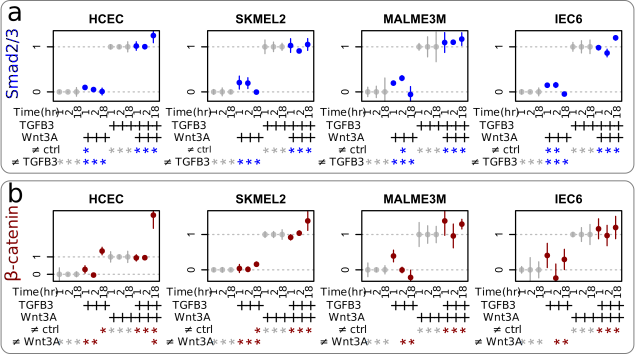
\includegraphics[width=6.5in]{FIGS/insulation/wntTgfbInsulation+.pdf}
  {\singlespacing 
  \caption[Wnt and \tgf\ are insulated during signal transduction (all data).]
        { Wnt and \tgf\ are insulated during signal transduction.
          \b{a}, Wnt3A causes little or no modulation of Smad2/3 responses at
          both short (1-2hr) and long (18hr) timepoints for all
          cell lines tested. \b{b}, \tgf 3 causes little or no
          modulation of \bcat\ responses, except in the case of
          long-term treatment in HCECs (note the 18hr \tgf 3 and 
          \tgf 3+Wnt3A responses). Y-axes and p-values as in
          \ar{fig:insulation:specificity}, with normalization per
          timepoint to set the control to 0 and the canonical-input-only
          condition to 1. These values fixed by normalization are in gray.
          $n=3$ replicates per point. p-values indicate
          whether each condition differs from control
          ($\neq$ctrl) or from the canonical-input-only
          condition (either $\neq$\tgf 3 or $\neq$Wnt3A).
          Concentrations (1 and 2hr): 0.2ng/mL \tgf 3,
          100ng/mL Wnt3A. Concentrations (18hr): 10ng/mL \tgf 3,
          200ng/mL Wnt3A.
          }
  \label{fig:insulation:wntTgfbInsulation}}
  \end{figure}
  

  \begin{figure}[!bt]
  \centering
  \includegraphics[width=5in]{FIGS/insulation/wntTgfb_summary.pdf}
  {\singlespacing 
  \caption[Wnt and \tgf\ are insulated during signal transduction (summary).]
        { Summary figure for insulation between Wnt3A and \tgf 3,
          limited to SKMEL2s and HCECs at 2 and 18hrs.
          \b{a}, At 2hrs, there is complete signaling insulation between
          Wnt3A and \tgf 3.
          \b{b}, However, context-dependent transcriptional integration
          already occurs at the same timepoint: HCECs show inhibition of
          Axin2 mRNA expression by \tgf 3 treatment, while SKMEL2s show
          complete transcriptional insulation.
          \b{c}, This context-dependent effect shows up at the level
          of signaling hours later, in HCECs. The increase in \bcat\ due
          to \tgf 3 signaling likely stems from the inhibition of Axin2
          mRNA (since Axin2 is a negative auto-regulator of Wnt3A). Thus,
          signaling insulation (\b{a}) combined with transcriptional integration
          (\b{b}) leads to a new, biased signaling state over time (\b{c}).
          Daggers
          indicate significant departure from pathway insulation.
          Data for \b{a} and \b{c} from \ar{fig:insulation:wntTgfbInsulation}.
          Data for \b{b} from \ar{fig:insulation:expressionXtalk}.
          }
  \label{fig:insulation:wntTgfbSummary}}
  \end{figure}
    

  
To test this, I treated all four cell types with combinatorial
inputs of \tgf 3 and Wnt3A, and then measured nuclear accumulation
of the transcription factors Smad2/3 and \bcat\ by
single-cell image analysis.
Data for all four cell lines are shown for 1, 2, and 18hr timepoints in
\arp{fig:insulation:wntTgfbInsulation}. This is a lot of data, and so
for simplicity I refer the reader to \ar{fig:insulation:wntTgfbSummary}, which shows
only the essential data for HCECs and SKMEL2s.


I performed the initial experiment at 1 and 2hr timepoints, using
ligand concentrations that ranged from EC50 to saturating across
the cell lines. In all cases, Wnt3A had small or
statistically insignificant effects on Smad2/3 levels, even when 
co-treated with \tgf 3 (\ar{fig:insulation:wntTgfbInsulation}a,
1 and 2hr timepoints; \ar{fig:insulation:wntTgfbSummary}a, top).
The small Wnt3A-induced Smad2/3 increases may be
real, but are likely due to the trace contamination discussed earlier
(see \ar{fig:insulation:contamination}). 
The same absence of signaling integration occurs in the other direction,
from \tgf 3 to \bcat\ (\ar{fig:insulation:wntTgfbInsulation}b,
1 and 2hr timepoints; \ar{fig:insulation:wntTgfbSummary}a, middle).
In this case, the presence of \tgf 3 had no significant effects
on \bcat\ levels in any context. Therefore, Wnt3A and \tgf 3 
are completely insulated during signal transduction
(\ar{fig:insulation:wntTgfbSummary}a, bottom).


Because the literature is full of examples of these two pathways interacting
over longer timescales, I decided to repeat the experiment with a more distant
timepoint.
To ensure that the absence of crosstalk was not due to low activity of the
pathways.
To my surprise, even at 18 hours there was almost no measurable modulation
of the transcription factor activity of one pathway by the other
(\ar{fig:insulation:wntTgfbInsulation}, 18hrs). There was
one exception, however: HCECs show \tgf 3$\rightarrow$\bcat\ interaction
(\ar{fig:insulation:wntTgfbSummary}c, middle). Indeed,
\tgf 3 treatment alone was sufficient to activate \bcat, and co-treatment
with Wnt3A yielded an approximately additive effect.


The complete absence of cross-pathway transcription factor modulation
at early timepoints strongly suggests that the Wnt3A and \tgf 3
signaling cascades are completely insulated from one another,
displaying no signaling crosstalk whatsoever
(\ar{fig:insulation:wntTgfbSummary}a, bottom). Further,
the frequent absence of cross-pathway modulation even given significant
time for transcriptional feedback shows that pathway insulation can be
maintained even after the transcriptional network has been remodeled by
morphogenic signals. Finally, the fact that HCECs lose this insulation
at later timepoints demonstrates a case of context-dependency
(i.e. dependency on cell type) in cellular decision-making
despite context-independent insulation of signal transduction
(\ar{fig:insulation:wntTgfbSummary}c, bottom).

  
\subsection{Wnt and \tgfbsf\ show context-dependent transcriptional integration}
 

Due to the surprising result that the direct outcomes of signaling
(transcription factor levels) are completely insulated between Wnt3A and \tgf 3,
I decided to test for insulation at the level of transcription. By
measuring mRNA expression 2hrs after treatment, I reasoned that I could
identify whether insulation at the level of signaling (as
already demonstrated) necessarily
implies insulation at the level of transcription. Because Axin2 and
Smad6/7 are the only prototypical transcription targets of the \tgfbsf\
and Wnt pathways, I measured mRNA levels of these genes following
combinatorial ligand treatment (\ar{fig:insulation:expressionXtalk};
simplified in \ar{fig:insulation:wntTgfbSummary}b).
 
 
  \begin{figure}[!bt]
  \centering
  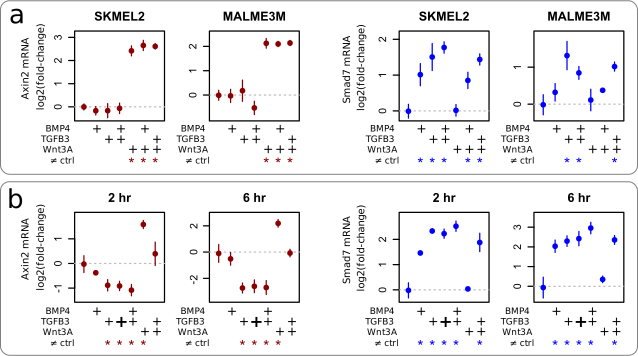
\includegraphics[width=6in]{FIGS/insulation/expressionXtalk.pdf}
  {\singlespacing 
  \caption[ Wnt and TGFB show context-dependent transcriptional crosstalk.]
        { Wnt and TGFB show context-dependent transcriptional crosstalk.
          \b{a}, In the melanoma cell lines, \tgf 3/BMP4 have no effect on
          Axin2 expression, while Wnt3A treatment has no effect on
          Smad7 expression. 2hr treatment.
          \b{b}, In HCECs, \tgf 3 reduces baseline and blocks
          Wnt3A-induced Axin2 expression. This effect is already apparent
          at 2hrs and is maintained at 6hrs. Wnt3A does not affect
          Smad7 expression in any context. Bold `+' indicates doubled
          \tgf 3 concentration, demonstrating transcriptional saturation of this pathway.
          Fold-change is relative to the control condition.
          Mean and standard deviation
          of 3 replicates, `*' indicates two-tailed p-value <0.05
          (Student's t-test).
          Concentrations: 10ng/mL \tgf 3, 25ng/mL BMP4, 200ng/mL Wnt3A.
          See \nameref{insulation:methods} for qPCR details.
        }
  \label{fig:insulation:expressionXtalk}}
  \end{figure}
  

By qPCR, neither of the melanoma cell lines show transcriptional
crosstalk between the canonical \tgfbsf\
and Wnt3A outputs Smad7 and Axin2
(\ar{fig:insulation:expressionXtalk}a), implying that these pathways
are insulated both in terms of the quantity of the transcription factors
sent to the nucleus (as shown in \ar{fig:insulation:wntTgfbInsulation})
and in the general activity of those
transcription factors. (This is not to say that these transcription factors
do not affect one another for any transcriptional targets.)
However, as before, HCECs display a different behavior.
By 2 hours HCECs show strong modulation of Axin2 expression
by \tgf 3 treatment(\ar{fig:insulation:wntTgfbSummary}b),
and this effect increases over time
(\ar{fig:insulation:expressionXtalk}b).


The modulation of Axin2 by \tgf 3 in HCECs is intriguing for
several reasons. First, it provides a simple explanation for the
18hr transcription factor modulation result observed in
(\ar{fig:insulation:wntTgfbSummary}c), since repression of Axin2,
a negative autoregulator of \bcat, could block the negative feedback
otherwise present after Wnt3A stimulation. Second, it clearly
shows that HCECs can simultaneously display signaling insulation
and transcriptional crosstalk,
demonstrating that these two processes can be completely
independent. Finally, the general lack of crosstalk across all
cell lines, coupled with the single instance of transcriptional
crosstalk in HCECs, is suggestive that the oft-cited idiosyncratic
outcomes of Wnt/\tgfbsf\ crosstalk are predominantly due to
context-dependent transcriptional crosstalk.

